
\begin{frame}{Points d'intérêts}
\note{
Pour un objet convexe tel qu'un cube, il nous suffit de répérer ces sommets pour le reconstruir en 3D.
Mais si l’objet est non convexe, comme dans le schéma de droite, on peut détecter des coins qui ne sont pas représentatifs de la structure globale.
On voit ici que l’enveloppe convexe (en bleu) ne correspond pas exactement à la forme réelle. Ce genre de situation peut gêner certaines étapes de reconstruction.
}
\begin{minipage}[t]{0.48\textwidth}
\centering
\textbf{Points d'intérêts  sur un cube}\\[0.5em]
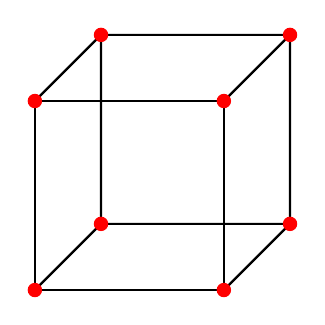
\begin{tikzpicture}[scale=1.2]

% Cube en perspective
\coordinate (A) at (0,0);
\coordinate (B) at (2,0);
\coordinate (C) at (2,2);
\coordinate (D) at (0,2);
\coordinate (E) at (0.7,0.7);
\coordinate (F) at (2.7,0.7);
\coordinate (G) at (2.7,2.7);
\coordinate (H) at (0.7,2.7);

% Faces du cube
\draw[thick] (A) -- (B) -- (C) -- (D) -- cycle; % face avant
\draw[thick] (A) -- (E) -- (F) -- (B); % face basse
\draw[thick] (B) -- (F) -- (G) -- (C);
\draw[thick] (C) -- (G) -- (H) -- (D);
\draw[thick] (D) -- (H) -- (E) -- (A);

\pause
% Coins détectés
\foreach \pt in {(A), (B), (C), (D), (E), (F), (G), (H)} {
  \filldraw[red] \pt circle (2pt);
}

\end{tikzpicture}
\end{minipage}
\hfill
\begin{minipage}[t]{0.48\textwidth}
\centering
\only<2->{
\pause
\textbf{Problème si non convexe}\\[0.5em]
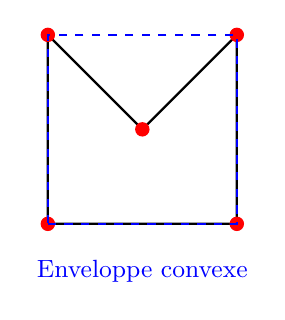
\begin{tikzpicture}[scale=1.2]
% Objet non convexe
\draw[thick] (0,0) -- (2,0) -- (2,2) -- (1,1) -- (0,2) -- cycle;

\pause
% Coins détectés
\foreach \pt in {(0,0), (2,0), (2,2), (1,1), (0,2)} {
  \filldraw[red] \pt circle (2pt);
}

\pause
% Enveloppe convexe
\draw[blue, dashed, thick] (0,0) -- (2,0) -- (2,2) -- (0,2) -- cycle;
\node[blue] at (1,-0.5) {\small Enveloppe convexe};
\end{tikzpicture}
}
\end{minipage}

\end{frame}

%===========================
\subsection{Filtrage epipolaire}
%===========================

\begin{frame}{Geometrie epipolaire}
\note{J’introduis ici la géométrie épipolaire : lorsque deux caméras observent une même scène, les points correspondants sont contraints de vérifier une relation géométrique.
Les deux caméras ont pour centres optiques respectifs C1 et C2 et pour plans-images P1 et P2. Pour des raisons de lisibilité, les plans-
images sont placés dans ce schéma devant les centres optiques. Un point M de la scène
se projette sur le plan-image de la caméra 1 (resp. 2) en m1 (resp. m2). Le point e1
(resp. e2) est l’image de C2 (resp. C1) sur P1 (resp. P2). Les points e1 et e2 sont appelés
épipoles. La droite l1 (resp. l2) joignant les points e1 et m1 (resp. e2 et m2) est appelée
droite épipolaire associée à m2 (resp. m1).
C’est cette contrainte qui nous permettra de filtrer les correspondances incorrectes.
Elle est encodé sous forme d'une matrice qu'on détermine à l'étape de calibration expliquéé ultérieurement}
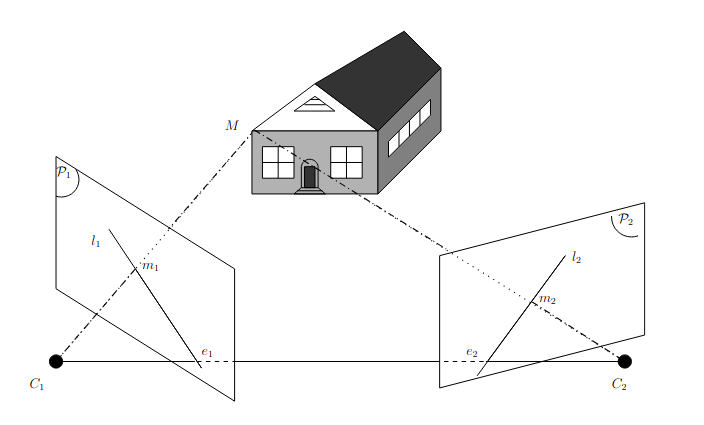
\includegraphics[width=\linewidth]{capture/geom-epipolaire.png}\\[0.5em]
\tiny
Source image: Quelques problèmes géométriques
en vision par ordinateur - Frédéric SUR
\end{frame}

\begin{frame}{Filtrage epipolaire}
  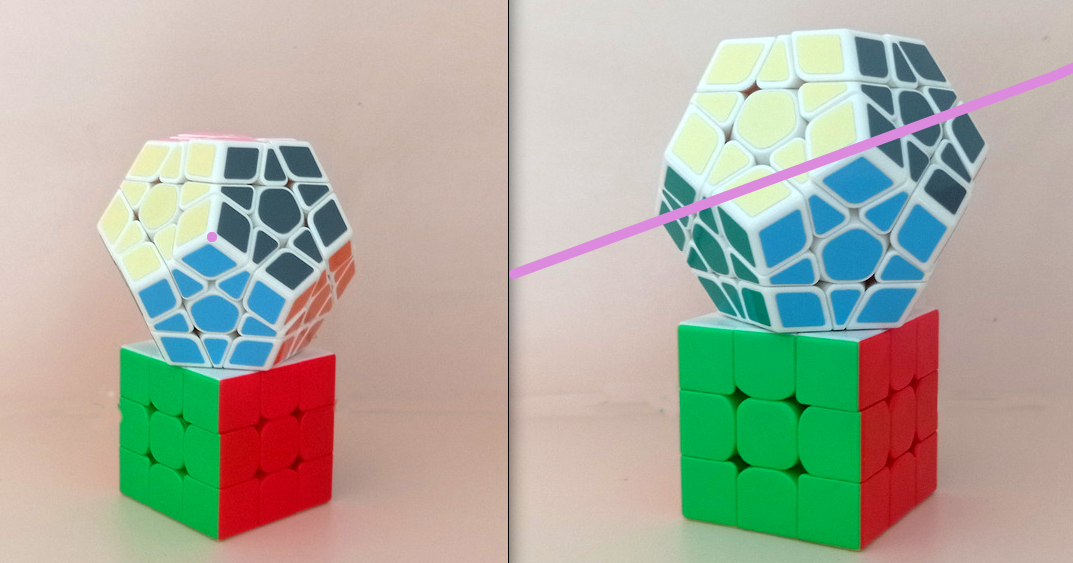
\includegraphics[width=\linewidth]{capture/ligne.png}\\[0.5em]
  \captionof*{figure}{Droite epipolaire}
\end{frame}

\begin{frame}{Résultats pré-traitement}

    \begin{center}
    \begin{minipage}{0.32\textwidth}
        \onslide<1->{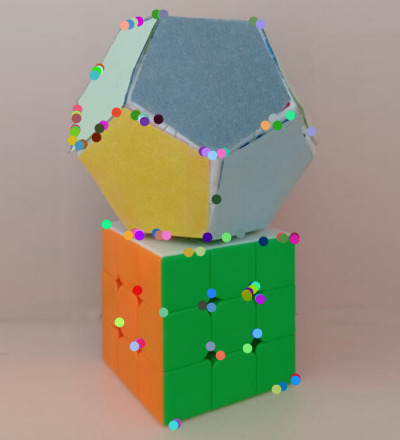
\includegraphics[width=\linewidth]{capture/app_complet_1.jpeg}\\
        \centering\scriptsize Points gardés}
    \end{minipage}
    \hfill
    \begin{minipage}{0.64\textwidth}
        \onslide<2->{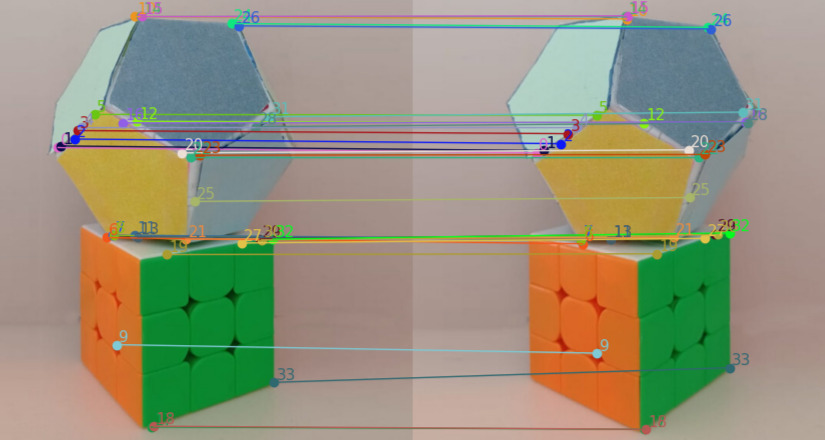
\includegraphics[width=\linewidth]{capture/app_complet_2.jpeg}\\
        \centering\scriptsize Appariement}
    \end{minipage}
    \end{center}
    \appxnote{constantes}{Appariement:\\
int Distance_seuil = 4;
int Hamming_seuil = 45;\\ \\

Detection\\
int Window = 4;
int Seuil_moravec = 800;\\


Ransac \\
int RANSAC_ITER = 1000;
int DIST_THRESHOLD=1.0;
int MIN_INLIERS=5;\\\\

Trouve coin\\
int Seuil_tc =40;
int Dist_tc = 10;
}